

Camera calibration is the process of finding the quantities internal to the camera that affect the imaging process. Today's cheap camera lenses or camera production errors may introduce a lot of distortion to images. Precise camera calibration is important when we need to deal with 3D interpretation of images, reconstruction of world models, and robot interaction with the real world. We will apply what we have learnt so far to discover the charm of camera calibration and its usage in our project.
\section{Preliminaries: Geometrical Transformations}
\subsection{Homogeneous Coordinates}
Homogeneous coordinates are widely used in computer vision and graphics. They are a nice extension of standard 3D vectors and allow us to simplify and compute various vector operations, such as translation, rotation, scaling and perspective projection. The sequence of such operations can be multiplied out into a single matrix with simple and efficient processing.Besides, homogeneous coordinates also allow to represent infinity. The Euclidean coordinate system denotes the location of an object by a triplet of numbers. However, we can't treat infinity as a regular number. Homogeneous coordinates allows by denoting infinity by $[x, y, z, 0] = \frac{[x, y, z]}{0}$ in 3D. \\
\begin{tcolorbox}[sharp corners, colback=green!30, colframe=green!80!blue, title=\textbf{\large How to transfer between Cartesian Coordinates and Homogeneous Coordinates?}]
\begin{itemize}
    \item Cartesian coordinates $\rightarrow$ Homogeneous coordinates : Multiply the coordinates by a non-zero scalar and add an extra coordinate equal to that scalar. For example, $[x,y] \rightarrow [x\cdot z, y\cdot z, z], z\neq0$.  
  We usually multiply the coordinates by 1.
  \item  Homogeneous coordinates $\rightarrow$ Cartesian coordinates:
  Divide the Cartesian coordinates by the last coordinate and eliminate it. For example, $[x, y, z], z\neq 0 \rightarrow [x/z, y/z]$.
\end{itemize}
\end{tcolorbox}

\subsection{2D Translation}
\begin{figure}[h!]
\centering
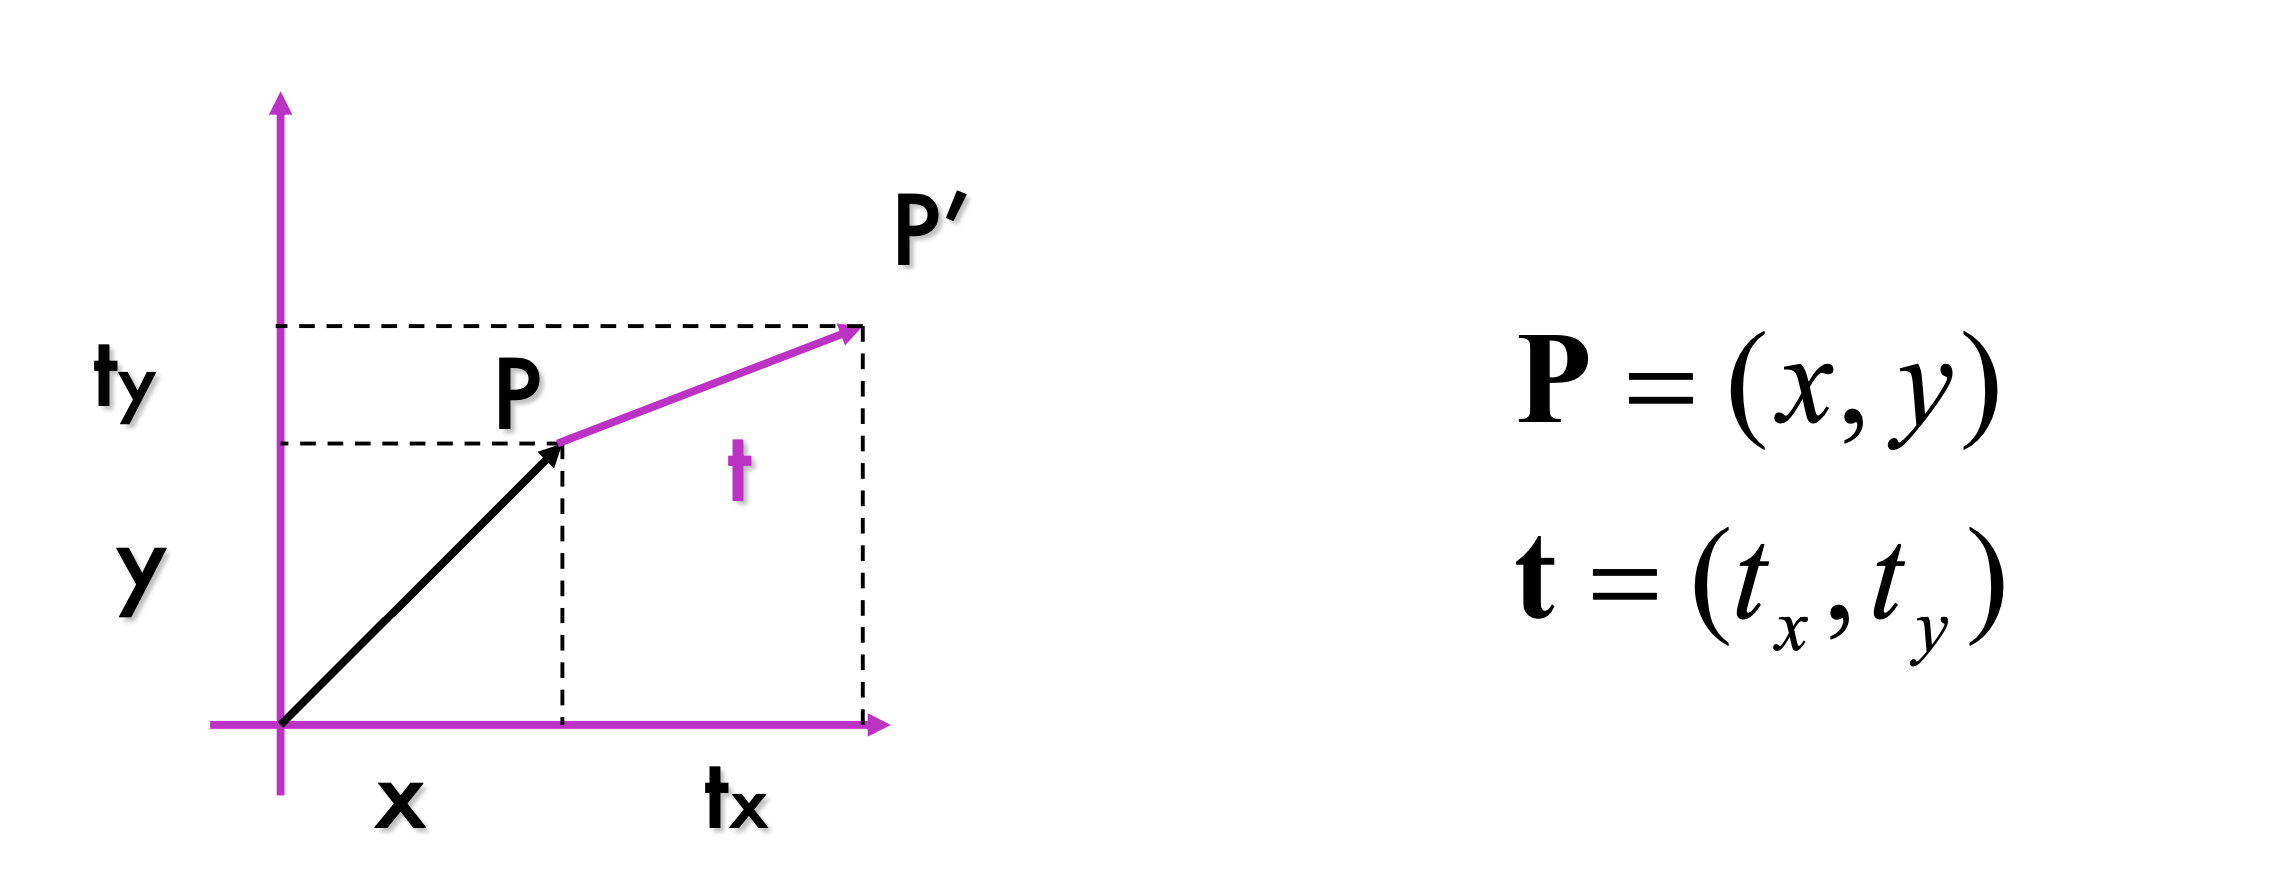
\includegraphics[width=0.6\textwidth]{graphicsAppendices/2D_Transformation.png}
\caption{Example of 2D Translation}
\label{fig:2DTranslation}
\end{figure}
If point $\textbf{P'}(x', y')$ is obtained by translating \textbf{P} by $\textbf{t}(t_x, t_y)$, then the relation between \textbf{P'} and \textbf{P} could be written as:\\
$$\textbf{P'} = \left[\begin{array}{c} x+t_x \\ y+t_y \end{array}\right] = \left[\begin{array}{ccc} 1 & 0\\ 
0 & 1 \end{array}\right]\left[\begin{array}{c} x \\ y \end{array}\right] +  \left[\begin{array}{r}t_x \\ t_y\end{array}\right] = \textbf{I} \cdot \textbf{P} + \textbf{t}$$  
If we use homogeneous coordinates, $P = (x, y, 1)$, and $t=(t_x, t_y, 1)$. The the relation between $P'$ and $P$ becomes:
$$\textbf{P'} = \left[\begin{array}{r}x+t_x \\ y + t_y \\ 1 \end{array}\right] =  \left[\begin{array}{rrr} 1 & 0 & t_x\\ 0 & 1 & t_y\\ 0 & 0 & 1 \end{array}\right] \left[\begin{array}{r}x\\ y\\ 1 \end{array}\right] =  \left[\begin{array}{rr}\textbf{I} & \textbf{t} \\ 0 & 1 \end{array}\right]\cdot \textbf{P} = \textbf{T} \cdot \textbf{P}$$

\subsection{2D Scaling}
\begin{figure}[h!]
\centering
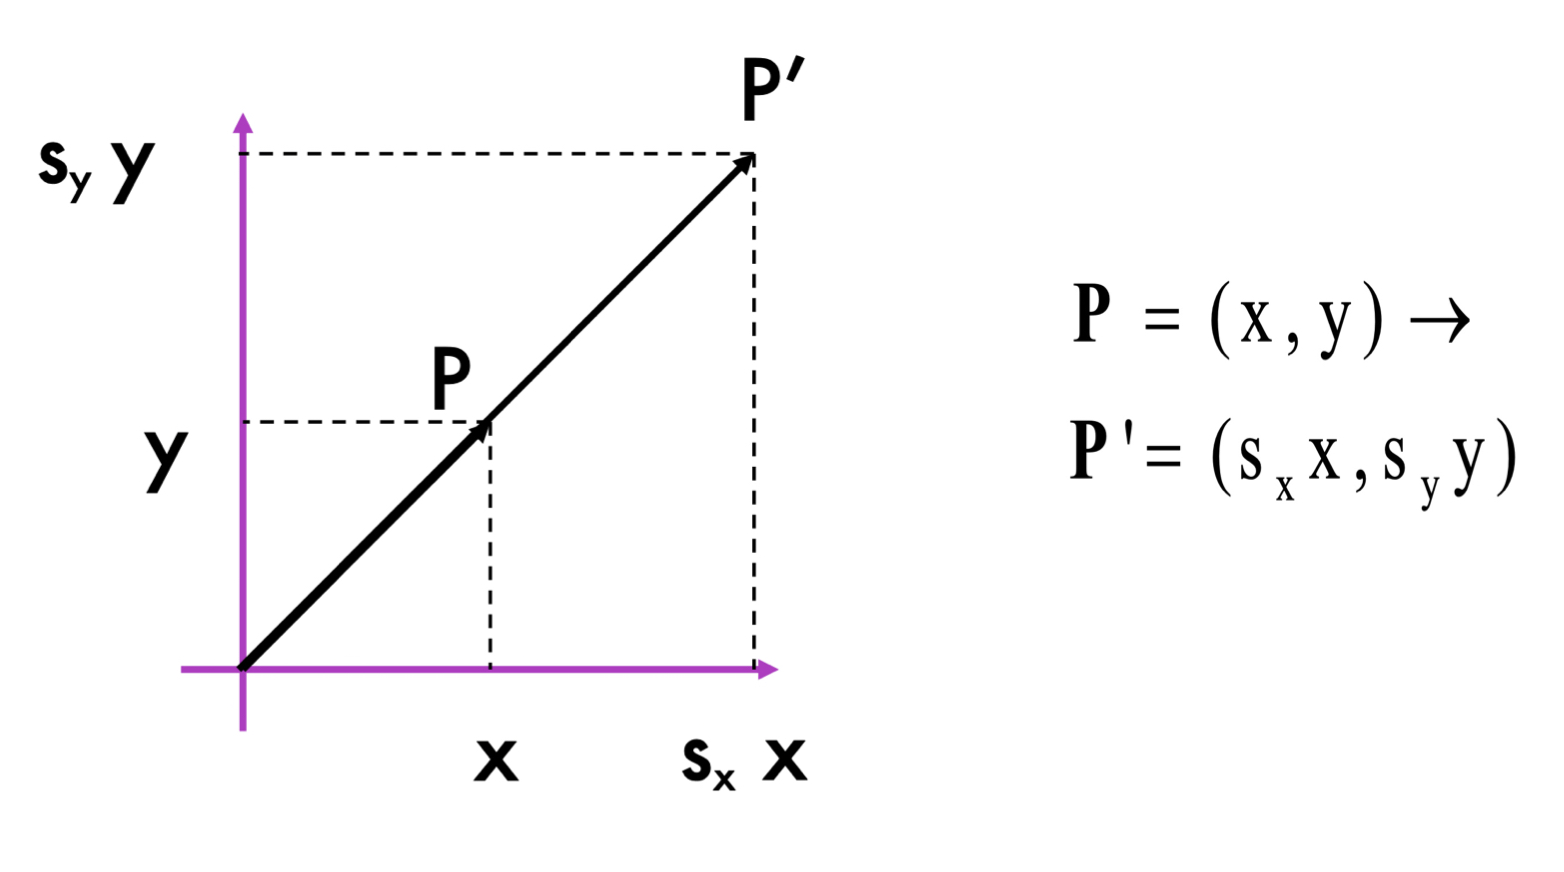
\includegraphics[width=0.4\textwidth]{graphicsAppendices/2D_Scaling.PNG}
\caption{Example of 2D Scaling}
\label{fig:2DScaling}
\end{figure}
If point $\textbf{P'}(x', y')$ is obtained by scaling \textbf{P} by $\textbf{s}(s_x, s_y)$, then the relation between \textbf{P'} and \textbf{P} could be written as:\\
$$\textbf{P'} = \left[\begin{array}{c} s_x x \\ s_y y \end{array}\right] = \left[\begin{array}{ccc} s_x & 0\\ 
0 & s_y \end{array}\right]\left[\begin{array}{c} x \\ y \end{array}\right] = \textbf{S'} \cdot \textbf{P}$$  
Similar before, the relation between \textbf{P'} and \textbf{P} could be expressed in homogeneous coordinates:
$$\textbf{P'}=\left[\begin{array}{c} s_{x} x \\ s_{y} y \\ 1 \end{array}\right] = \left[\begin{array}{ccc} s_x & 0 & 0 \\ 0 & s_y & 0 \\ 0 & 0 & 1 \end{array}\right] \left[\begin{array}{c} x \\ y \\ 1 \end{array}\right] = \left[\begin{array}{rr} \textbf{S'} & 0 \\ 0 & 1 \end{array}\right] \textbf{P} = \textbf{S} \cdot \textbf{P}$$

\subsection{2D Rotation}
\begin{figure}[h!]
\centering
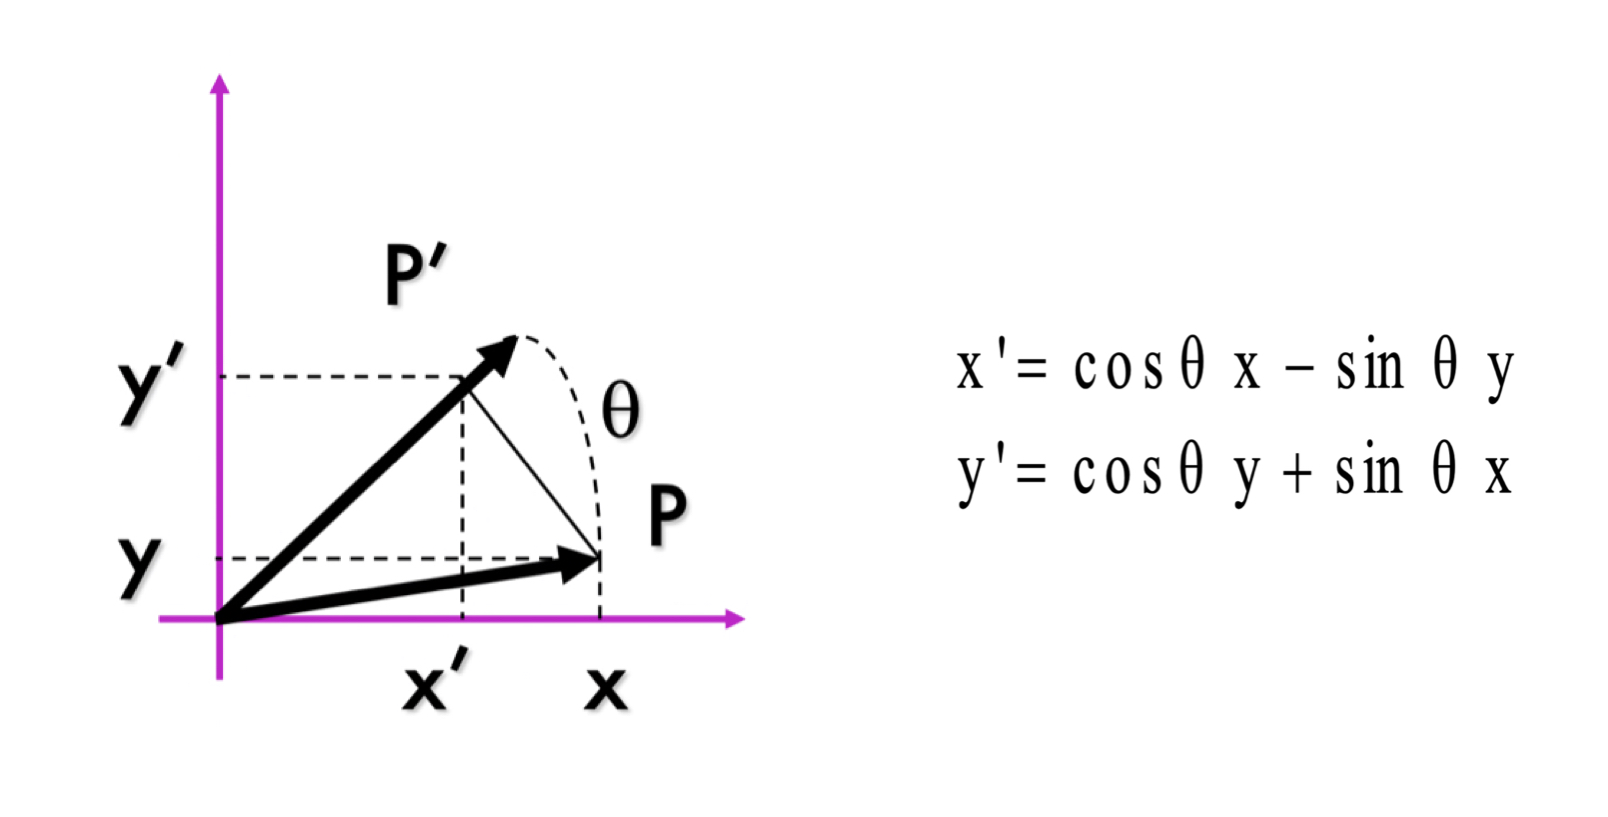
\includegraphics[width=0.5\textwidth]{graphicsAppendices/2D_Rotation.PNG}
\caption{Example of 2D Rotation}
\label{fig:2DRotation}
\end{figure}

If point $\textbf{P'}(x', y')$ is obtained by rotating \textbf{P} counterclockwise by $\theta$ degree, then the relation between \textbf{P'} and \textbf{P} could be written as:\\
$$\textbf{P'} = \left[\begin{array}{cc} \text{cos}\theta & -\text{sin}\theta \\ \text{sin}\theta & \text{cos}\theta\end{array}\right]\left[\begin{array}{c} x \\ y \end{array}\right] = \textbf{R'} \cdot \textbf{P}$$

The relation between \textbf{P'} and \textbf{P} could be expressed in homogeneous coordinates:
$$\textbf{P'}= \left[\begin{array}{ccc} \text{cos}\theta & -\text{sin}\theta & 0 \\ \text{sin}\theta & \text{cos}\theta & 0 \\ 0 & 0 & 1 \end{array}\right] \left[\begin{array}{c} x \\ y \\ 1 \end{array}\right] = \left[\begin{array}{rr} \textbf{R'} & 0 \\ 0 & 1 \end{array}\right] \textbf{P} = \textbf{R} \cdot \textbf{P}$$  
\begin{tcolorbox}
R is an orthogonal matrix and it satisfies the following properties:
\begin{itemize}
    \item $R \cdot R^\top = R^\top \cdot R = I$
    \item det(R) = 1
\end{itemize}
\end{tcolorbox}

\subsection{Other 2D Geometrical Transformations in Homogeneous Coordinates}
\begin{itemize}
    \item Shear in x: $ \left[\begin{array}{ccc} 1 & k_x & 0 \\ 0 & 1 & 0 \\ 0 & 0 & 1 \end{array}\right]$
    \item Shear in y: $ \left[\begin{array}{ccc} 1 & 0 & 0 \\ k_y & 1 & 0 \\ 0 & 0 & 1 \end{array}\right]$
    \item Reflect about y: $ \left[\begin{array}{ccc} 1 & 0 & 0 \\ k_y & 1 & 0 \\ 0 & 0 & 1 \end{array}\right]$
    \item General Affine Transformation: $ \left[\begin{array}{ccc} a & b & c \\ d & e & f \\ 0 & 0 & 1 \end{array}\right]$
\end{itemize}
\begin{tcolorbox}
If there are more than one type of geometric transformation, one can multiply the corresponding transformation matrix to get the final transformation matrix. \\
For example, if we want to find the transformation matrix after scaling P by s firstly, then rotating counterclockwise by $\theta$ degree, and finally translate by t. The position of P' could be compute by:
\begin{align*}
    P'= \textbf{T} \cdot \textbf{R} \cdot \textbf{S} \cdot P &=  \left[\begin{array}{rrr} 1 & 0 & t_x\\ 0 & 1 & t_y\\ 0 & 0 & 1 \end{array}\right]\left[\begin{array}{ccc} \text{cos}\theta & -\text{sin}\theta & 0 \\ \text{sin}\theta & \text{cos}\theta & 0 \\ 0 & 0 & 1 \end{array}\right]\left[\begin{array}{ccc} s_x & 0 & 0 \\ 0 & s_y & 0 \\ 0 & 0 & 1 \end{array}\right] \left[\begin{array}{r}x\\ y\\ 1 \end{array}\right] \\
    &= \left[\begin{array}{ccc} \text{cos}\theta & -\text{sin}\theta & t_x \\ \text{sin}\theta & \text{cos}\theta & t_y \\ 0 & 0 & 1 \end{array}\right]\left[\begin{array}{ccc} s_x & 0 & 0 \\ 0 & s_y & 0 \\ 0 & 0 & 1 \end{array}\right] \left[\begin{array}{r}x\\ y\\ 1 \end{array}\right]  \\
    &= \left[\begin{array}{cc} R' & t \\ 0 & 1 \end{array}\right]\left[\begin{array}{cc} S & 0 \\ 0 & 1 \end{array}\right] \left[\begin{array}{r}x\\ y\\ 1 \end{array}\right] \\
    &= \left[\begin{array}{cc} R'S & t \\ 0 & 1 \end{array}\right] \left[\begin{array}{r}x\\ y\\ 1 \end{array}\right] 
\end{align*}
\end{tcolorbox}

\section{Pinhole Model}
Last section we mainly discussed the affine transformation, which preserves the parallel lines, ratio of areas, ratio of lengths on colinear lines and a few others. However, the affine transformation is not a valid assumption in general for images, nor is it valid around the image edges. The mapping from 3D object to 2D image is a perspective projection as shown in the following image:

\begin{figure}[H]
\centering
\begin{minipage}{.4\textwidth}
  \centering
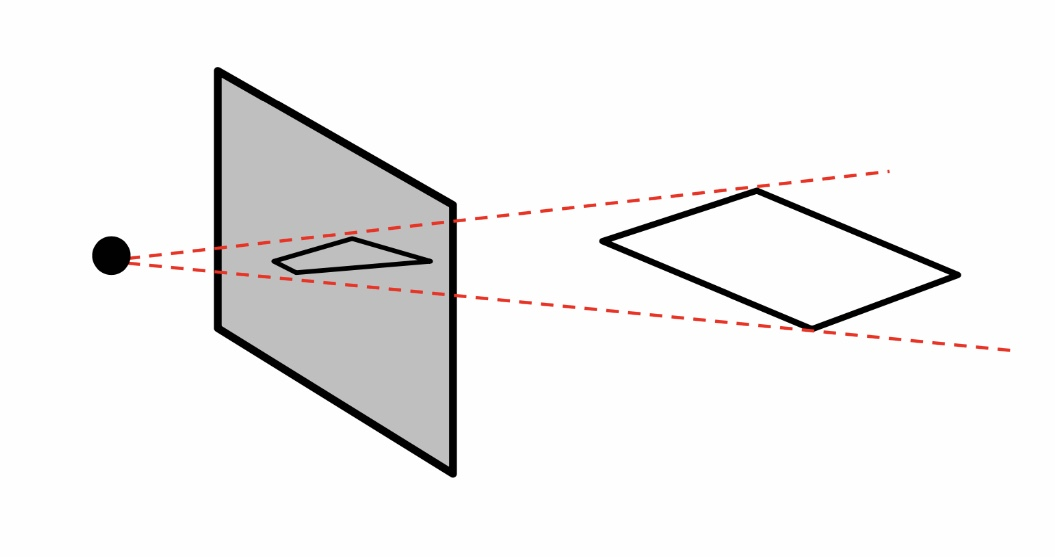
\includegraphics[width=\linewidth]{graphicsAppendices/perspective_diagram.png}
  \label{fig:perspectiveDiagram}
  \caption{Perspective schematic diagram}
\end{minipage}%
\hspace*{1cm}
\begin{minipage}{.4\textwidth}
  \centering
 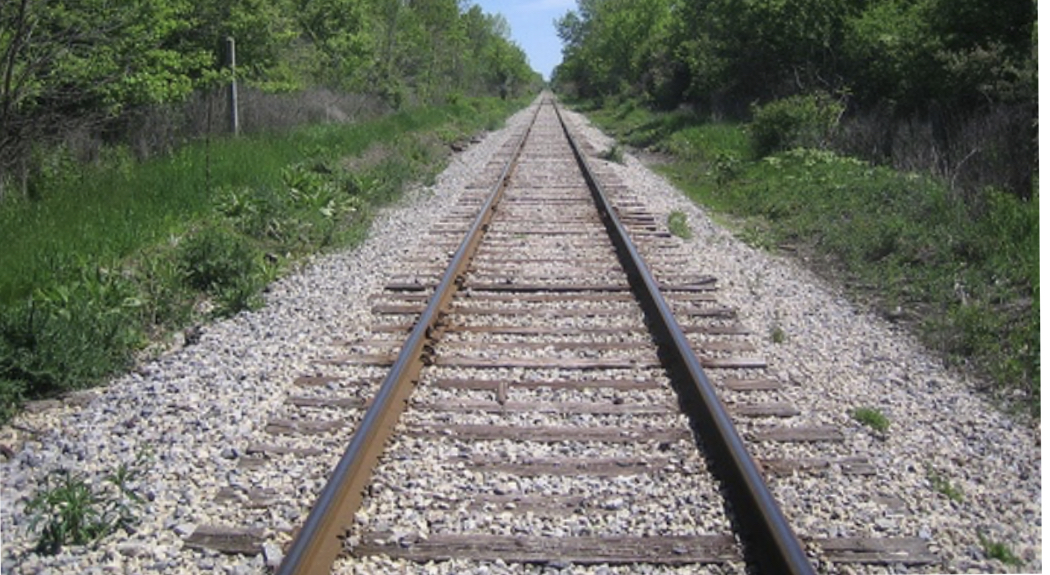
\includegraphics[width=\linewidth]{graphicsAppendices/perspective_rail.png}
 \caption{Real-life perspective example: parallel rails}
  \label{fig:perspectiveRail}
\end{minipage}
\label{fig:real-lifeExample}
\end{figure}
The \textbf{pinhole camera model} describes the mathematical relationship between the coordinates of a point in 3D space and its projection onto the image plane of an ideal pinhole camera. The following diagram illustrates the pinhole model and defines some intrinsic parameters of pinhole camera:
\begin{figure}[H]
\centering
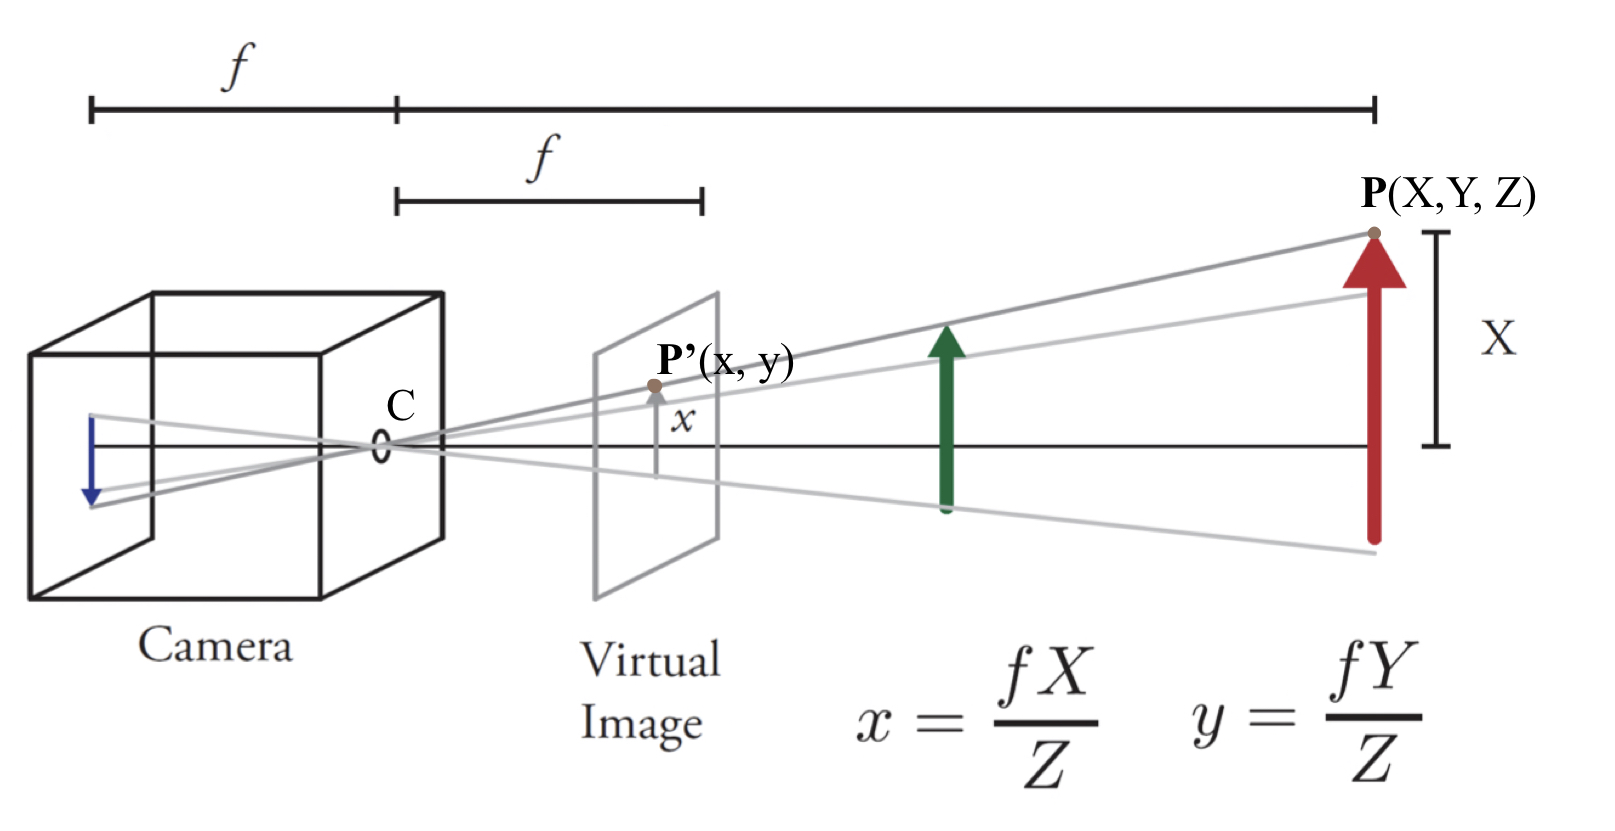
\includegraphics[width=0.6\textwidth]{graphicsAppendices/pinhole_camera.jpeg}
\caption{Pinhole camera model}
\label{fig:pinholeCameraModel}
\end{figure}

There are some key assumptions of the pinhole model:  
\begin{itemize}
    \item Aperture, i.e. the pinhole, is described as a point (point C in the image)
    \item No lenses are used to focus light, therefore no geometric distortions (radial distortion)
    \item Does not take into account that most practical cameras have only discrete image coordinates
    \item This model can only be used as a first order approximation of the mapping from 3D scene to 2D image. This is a perspective projection
    \item Ideal model that we use has identity matrix for the perspective portion of the projection matrix (\textbf{projection matrix} = $[\textbf{Perspective} | 0]$ = $[\textbf{I}_{3 \times 3} | 0]_{3 \times 4}$ which assumes no perspective since the surface is close to the camera)
\end{itemize}

If \textbf{P} $(X, Y, Z)$ is a 3D scene point, and it is projected into the 2D image by pinhole. \textbf{P'} $(x, y$ is the projective point of \textbf{P} on the 2D virtual image plane. We could find the following equations derived using similar triangles.  \\
\textbf{Remark}: f is the focal length of the camera.
\begin{figure}[H]
\centering
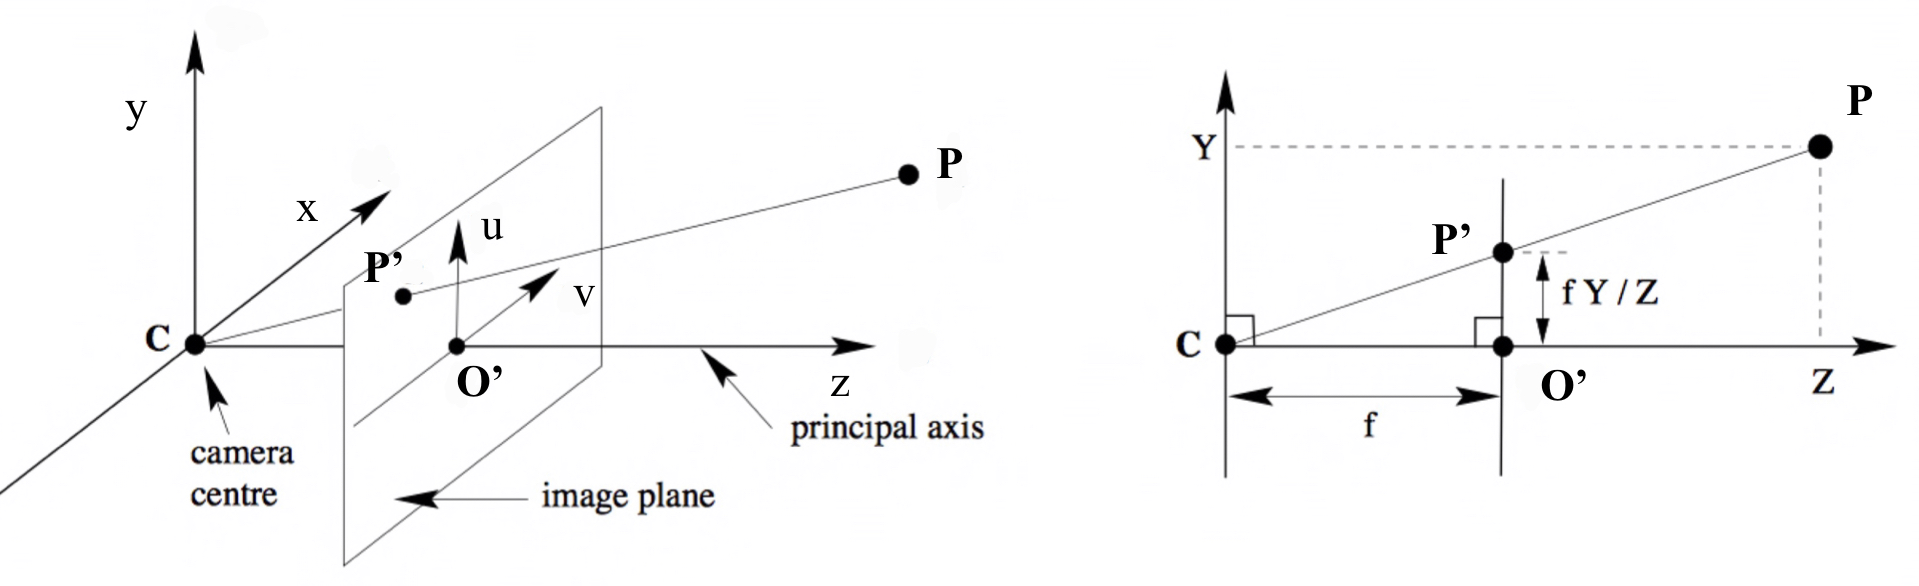
\includegraphics[width=0.8\textwidth]{graphicsAppendices/pinhole_model.jpeg}
\caption{Pinhole model}
\label{fig:pinholeModel}
\end{figure}
\begin{equation}
    \frac{f}{Z} = \frac{y}{Y} = \frac{x}{X} \implies \begin{cases} x = \frac{fX}{Z} \\ y=\frac{fY}{Z}\end{cases}
    \label{eq:relationCameraImage}
\end{equation}

The image plane is usually read as $n \times m$ pixel matrix in computer. Points in the image is then represented by pixel coordinates.
\begin{figure}[H]
\centering
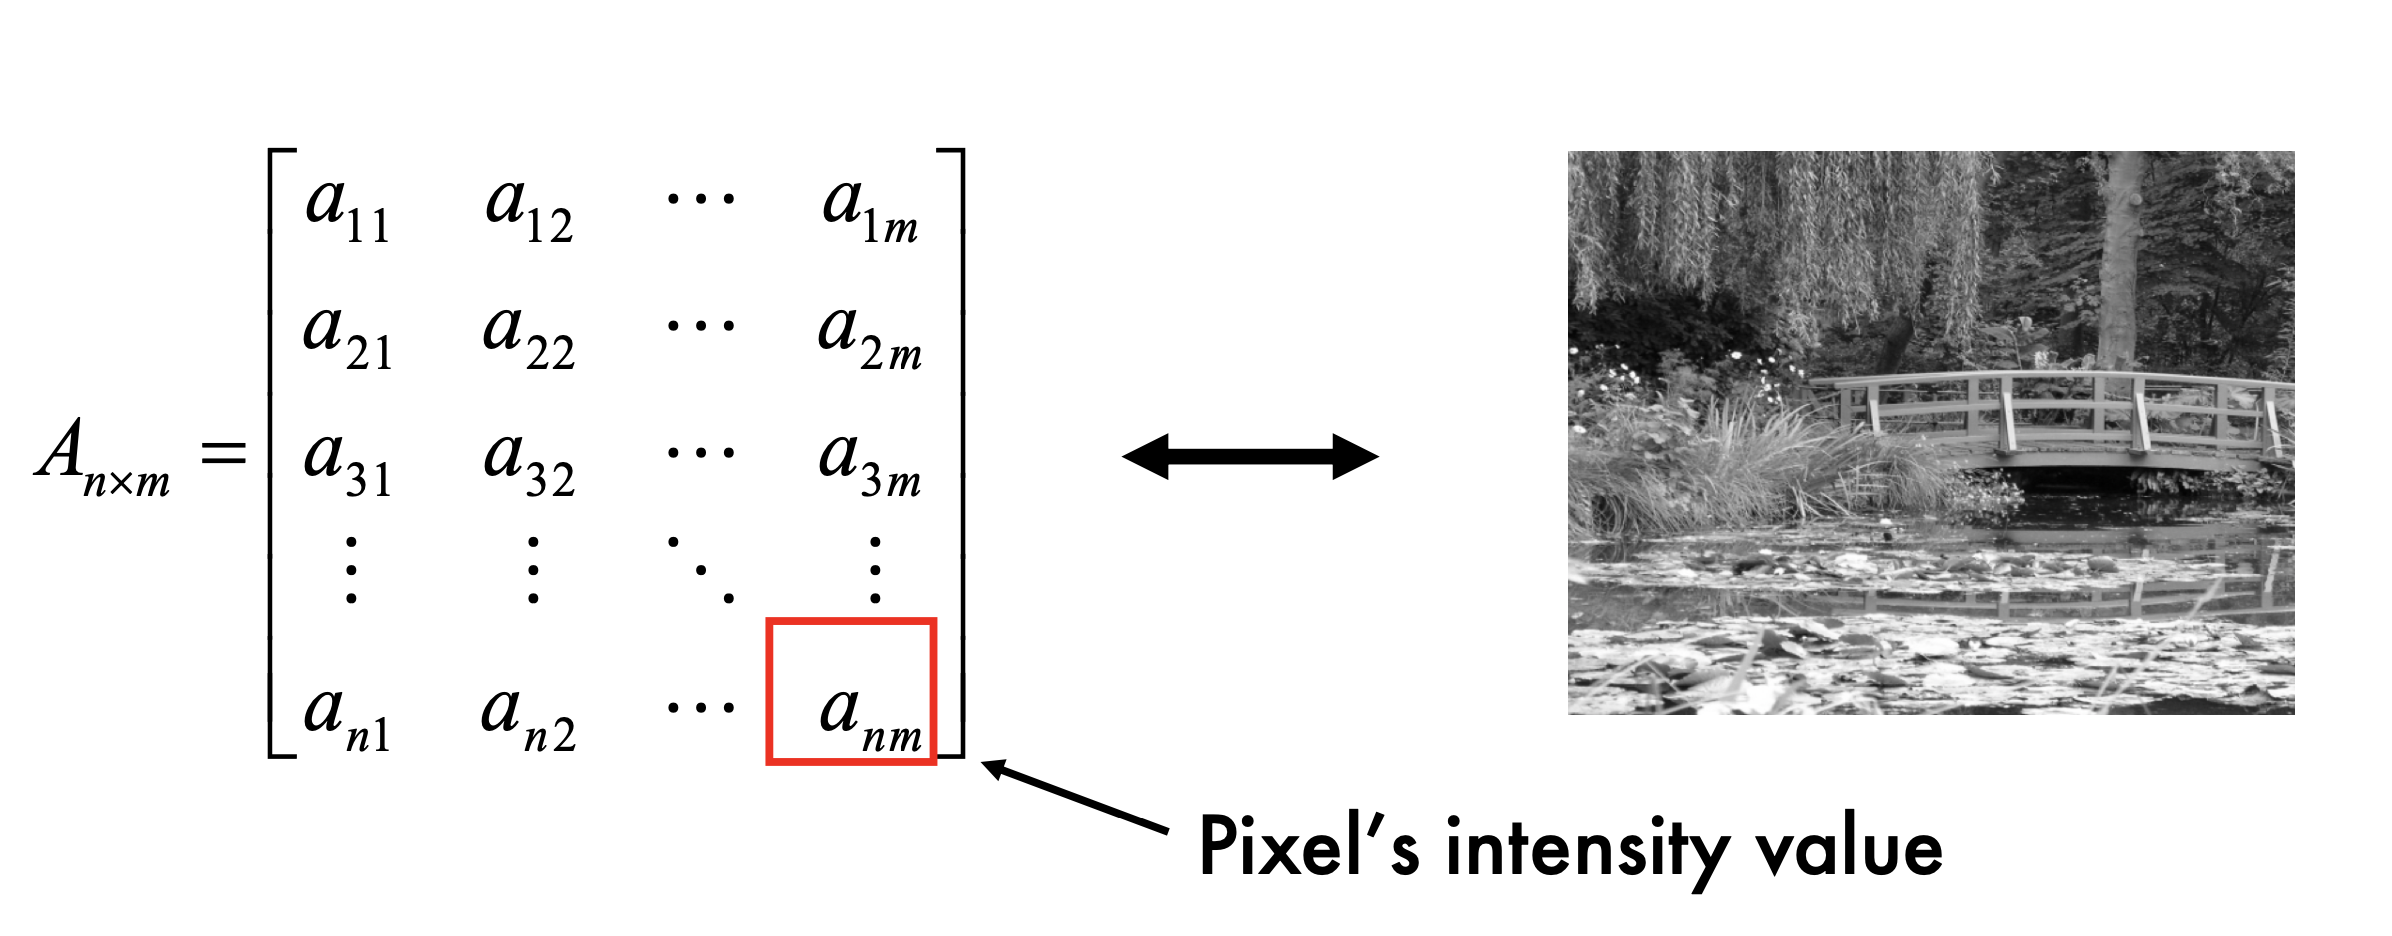
\includegraphics[width=0.8\textwidth]{graphicsAppendices/pixel.PNG}
\caption{Relation of image plane and pixel matrix}
\label{fig:pixelImage}
\end{figure}

The following picture is an example of image plane, which indicates the relation between camera coordinate origin and image coordinate origin

\begin{figure}[H]
\centering
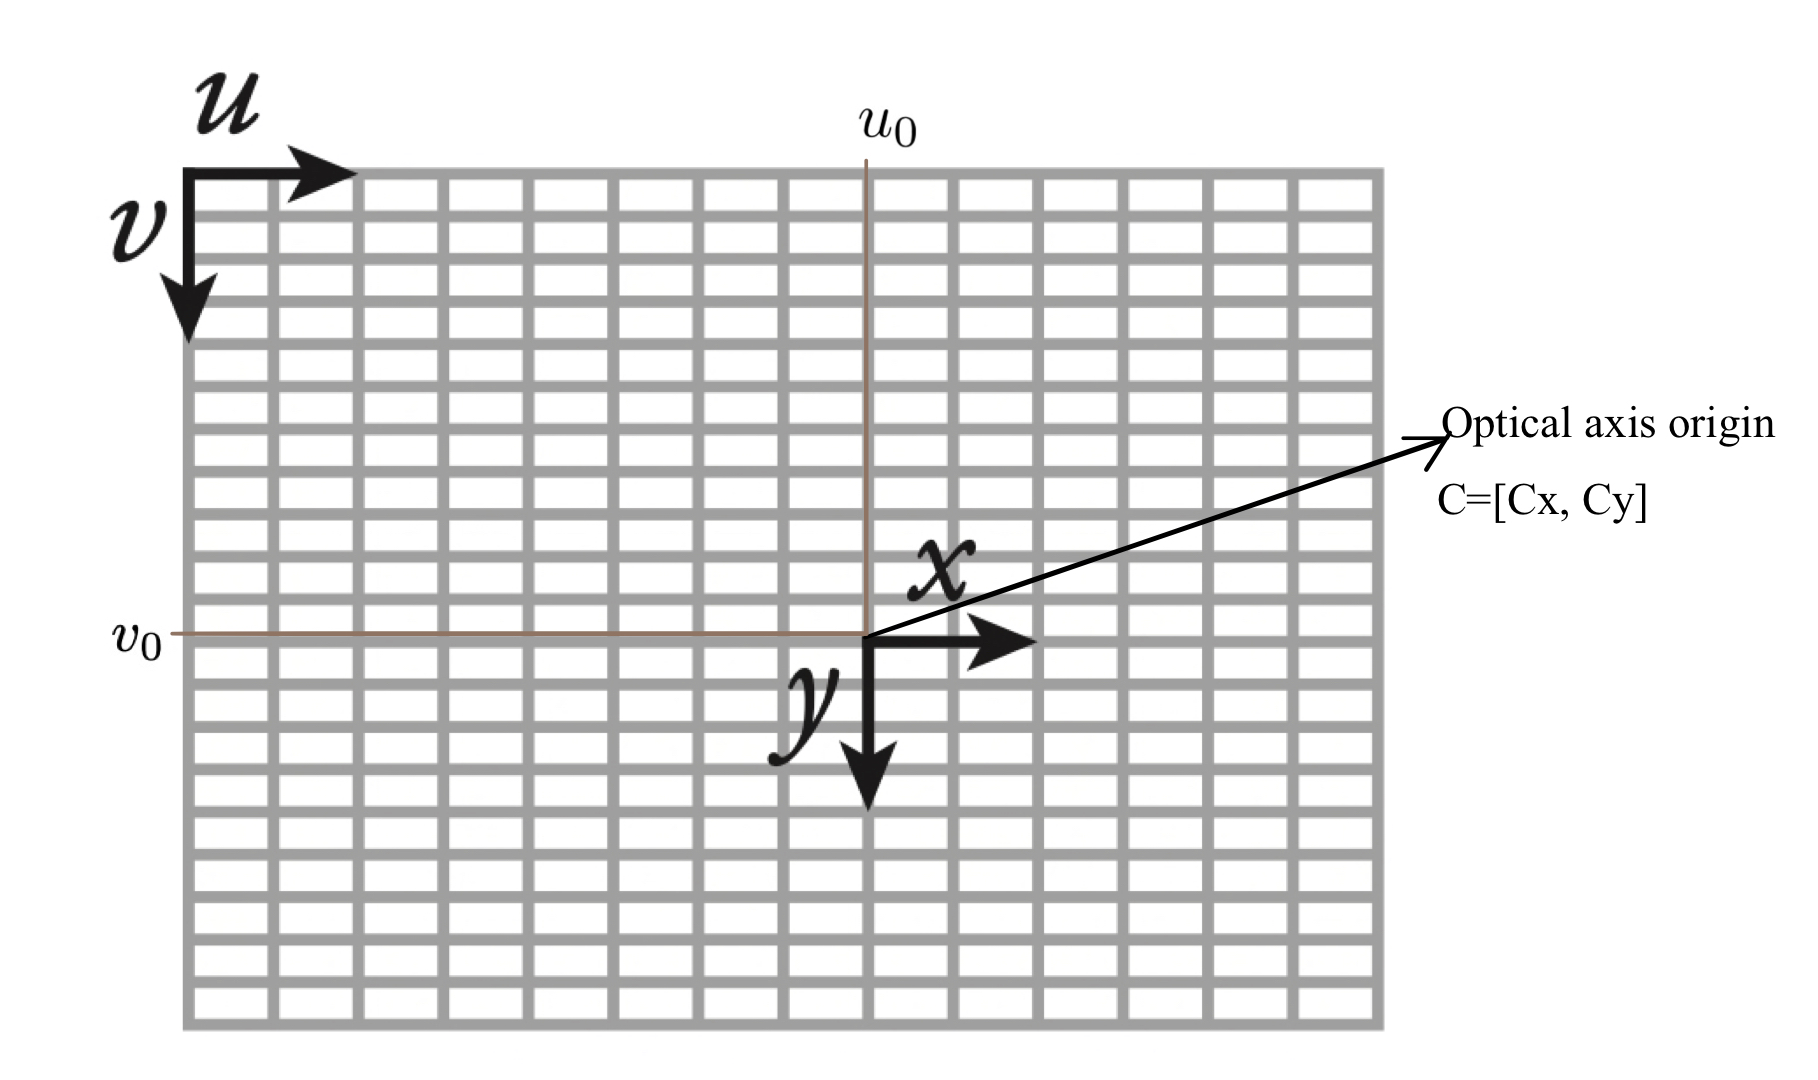
\includegraphics[width=0.5\textwidth]{graphicsAppendices/pixel_coordinates.jpeg}
\caption{Pixel coordinates plane}
\label{fig:pixelCoordinate}
\end{figure}

By expanding equation~\ref{eq:relationCameraImage}, the relation between positions on the image scene $(u, v)$ and positions in the real world $(X, Y, Z)$ could be written as:
\begin{align*}
 u &= f s_x x^c+u_0 = \alpha \frac{X}{Z} + u_0 \\
 v &= f s_y y^c+v_0 = \beta  \frac{Y}{Z} + v_0
 \end{align*}

We assume the world frame and camera frame is aligned. $s_x, s_y$ are the scale in x and y direction to transfer the units from metric to pixel. $x^c, y^c$ are projective points of 3D objects in camera coordinates. \\
\\
However, there are other considerations:
\begin{itemize}
    \item Optical axis is not centered on sensor
    \item Pixel coordinate system orgin is in the corner of the sensor
    \item Pixels aren't square
    \item Pixel size is unknown
\end{itemize}

Therefore, we need to find a transformation matrix to consider all the possible situations to transform the camera frame to the image plane. Review 2D geometric transformations in previous section and recall the general affine transformation $\left[\begin{array}{ccc} a & b & c \\ d & e & f \\ 0 & 0 & 1 \end{array}\right]$. We will explore more about it in the next section.

\section{Geometric and Mathematical Relations}
We would like to represent image plane coordinates in terms of real world coordinates. This is exactly the same problem as finding the conversion of 3D world coordinates to image coordinates and then inverting this transformation. In this section, we will examine the three components of this transformation. 

\subsection{Intrinsic Matrix K}
Intrinsic matrix is the affine transformation matrix we mentioned before to represent the linear properties of the pinhole camera model (focal length to visual image, scale, shear, translation, and so on). The intrinsic matrix can be used to transform 2D camera coordinates $(x^c, y^c)$ into image plane coordinates $(u, v)$:
$$\left[\begin{array}{c} u \\ v \\ 1 \end{array}\right] = K\left[\begin{array}{c} x^c \\ y^c \\ 1 \end{array}\right] = \left[\begin{array}{ccc} f s_x & k s_y & u_0 \\0 & f s_y & v_0 \\ 0 & 0 & 1 \end{array}\right]\left[\begin{array}{c} x^c \\ y^c \\ 1 \end{array}\right] = \left[\begin{array}{ccc} \alpha & s & u_0 \\0 & \beta & v_0 \\ 0 & 0 & 1 \end{array}\right]\left[\begin{array}{c} x^c \\ y^c \\ 1 \end{array}\right]$$
Where $s_x$ is the scale in x, $s_y$ is the scale in y, $f$ is the focal length, $k$ is the ration of shear in the y direction to that in x, and $(u_0, v_0)$ is the distance from the image center to the image plane coordinate system origin. 
\subsection{Projection Matrix}
This matrix transforms the coordinates from 3D to 2D. The perspective portion of this matrix (left) is equal to the identity because we make the assumption that all captured positions are close.
$$\left[\begin{array}{c}x^c\\y^c\\1\end{array}\right]=\frac{1}{Z_c}[P_{\text{perspective}} \quad 0]\left[\begin{array}{c}X^c\\Y^c\\Z^c\\1\end{array}\right]=\frac{1}{Z_c}[I_{3 \times 3} \quad 0]_{3 \times 4}\left[\begin{array}{c}X^c\\Y^c\\Z^c\\1\end{array}\right]$$
The positions are now shown in lower case and lie now on a 2D plane.

\subsection{Extrinsic Matrix }
This matrix belongs in SE(3) and it represents the transformation of position coordinates from the real world frame to the camera coordinate frame.
$$\left[\begin{array}{c}X^c \\ Y^c \\Z^c \\ 1 \end{array}\right] = [R \quad t]\left[\begin{array}{c}X \\ Y \\Z \\ 1 \end{array}\right]$$

\subsection{Full Projection Matrix Workspace to Camera}
Grouping everything together we get a final full projection matrix, P, such that
\begin{align*}
\left[\begin{array}{c}u \\ v \\ 1\end{array}\right]&=P\left[\begin{array}{c}X \\ Y \\ Z \\ 1\end{array}\right]\\
P &= K [I \quad 0][R \quad t] \\
&=\left[\begin{array}{ccc} \alpha & s & u_0 \\0 & \beta & v_0 \\ 0 & 0 & 1 \end{array}\right][I \quad 0][R \quad t]
\end{align*}
Or with the general affine transformation as the intrinsic matrix
$$P =\left[\begin{array}{ccc} a & b & c \\d & e & f \\ 0 & 0 & 1 \end{array}\right][I \quad 0][R \quad t]$$

\section{Intrinsic Matrix Calibration} 
Solve the simpler problem of only finding the intrinsic matrix if the extrinsic is known.  
If you are already given the 2D camera coordinates (post extrinsic and projective transformation, then you can select at least 3 known points in the real world and image plane (which do not all lie within the same plane). Remember the general form
$$\left[\begin{array}{c} u \\v \\ 1 \end{array}\right] =\left[\begin{array}{ccc} a & b & c \\d & e & f \\ 0 & 0 & 1 \end{array}\right]\left[\begin{array}{c} x^c \\y^c \\ 1 \end{array}\right]$$
For example, let's say that we know two different points then
$$\left[\begin{array}{c} u_1 \\v_1 \\ 1 \end{array}\right] =\left[\begin{array}{ccc} a & b & c \\d & e & f \\ 0 & 0 & 1 \end{array}\right]\left[\begin{array}{c} x^c_1 \\y^c_1 \\ 1 \end{array}\right], \quad \left[\begin{array}{c} u_2 \\v_2 \\ 1 \end{array}\right] =\left[\begin{array}{ccc} a & b & c \\d & e & f \\ 0 & 0 & 1 \end{array}\right]\left[\begin{array}{c} x^c_2 \\y^c_2 \\ 1 \end{array}\right]$$
The system of equations become
\begin{align*}
ax_1 + by_1+c &= u_1 \\
dx_1 + ey_1+f &= v_1 \\
ax_2 + by_2+c &= u_2 \\
dx_2 + ey_2+f &= v_2
\end{align*} 
Rearranging into the form $Ax=b$
$$\begin{bmatrix}  x_1 & y_1 & 1 & 0 & 0 & 0 \\ 0 & 0 & 0 & x_1 & y_1 & 1 \\ x_2 & y_2 & 1 & 0 & 0 & 0 \\ 0 & 0 & 0 & x_2 & y_2 & 1 \\ \vdots & \vdots &\vdots &\vdots &\vdots &\vdots \end{bmatrix}\left[\begin{array}{c} a \\ b \\ c \\d \\ e \\ f \end{array}\right]=\begin{bmatrix}  u_1 \\ v_1 \\ u_2 \\ v_2 \\ \vdots \end{bmatrix}$$
A quick and less rigorous derivation of the solution: We want to approximate $b$ with the subspace of $A$. This means through the projection theorem that $b-Ax$ is perpendicular to $Ax$
\begin{align*}
b-Ax &\perp Ax \\
(b-Ax) \cdot (Ax) &= 0 \\
(Ax) \cdot (Ax) &= (Ax) \cdot b \\
x^TA^TAx &= x^TA^Tb \\
x &= (A^TA)^{-1}A^Tb
\end{align*}
Then plug the corresponding values into the complete intrinsic matrix.

\section{Nonlinear Phenomena in Calibration}
In real life, because of the imperfect lens or inaccurate placement of the lens, the image would be distorted. We can use nonlinear root finding methods like Newton-Raphson to account for nonlinear phenomena. $(x_{distorted} = x_{linear} + g(x)$ \\
\begin{itemize}
    \item Radial Distortion\\
    This phenomenon occurs when light rays bend more near the edges of a lens than they do at this optical center. Smaller lens can lead to greater distortion.
    \begin{figure}[H]
    \centering
    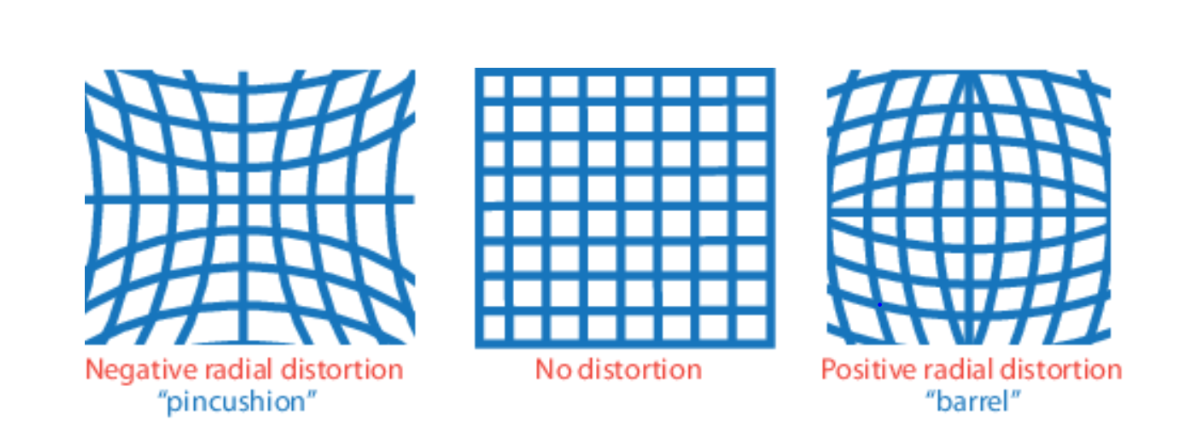
\includegraphics[width=0.6\textwidth]{graphicsAppendices/radial_distortion.PNG}
    \caption{Types of radial distortion}
    \label{fig:radialDistortion}
\end{figure}

    \item Tangential Distortion
    This phenomenon occurs when the lens and the image plane are not parallel
    \begin{figure}[H]
    \centering
    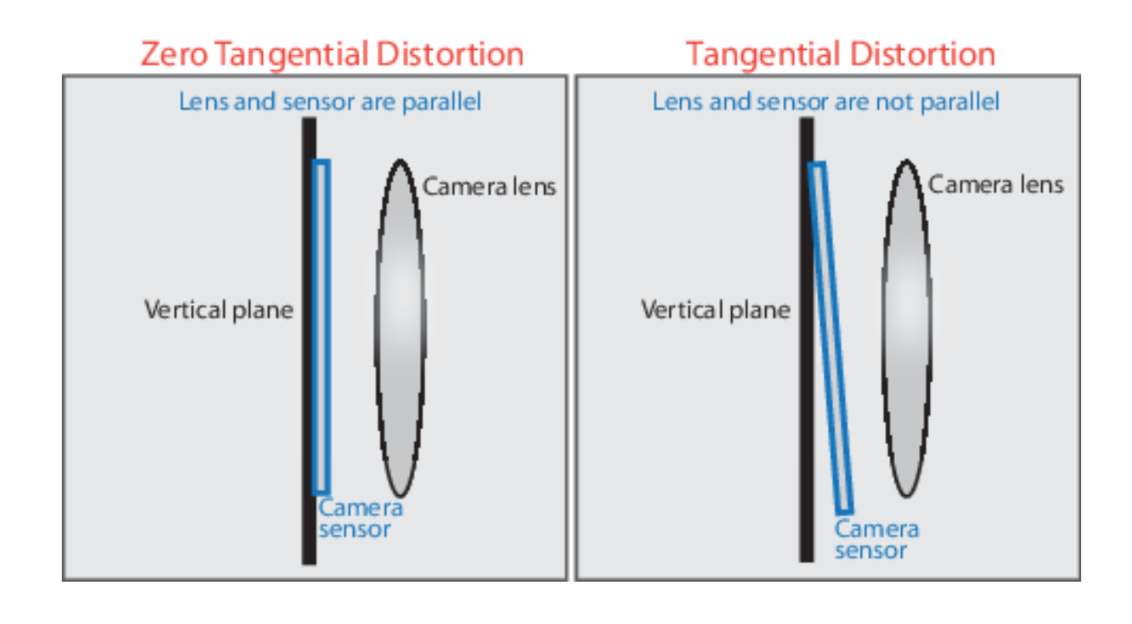
\includegraphics[width=0.6\textwidth]{graphicsAppendices/tangential_distortion.PNG}
    \caption{Tangential distortion}
    \label{fig:tangentialDistortion}
    \end{figure}
\end{itemize}